\section{\infersent{}}\label{sec:evaluation-inferSent}

% pool type
The \texttt{max} pooling type is used for the \infersent{} model, since the \citeauthor{inferSent2018} 
found from conducting experiments using different pooling techniques
that it was the best option.

% version/ embeddings dictionary
Initially, in this work, the \ac{glove} word embeddings were used for the \infersent{} model.
However, since the file of precomputed \acs{glove} word embeddings has a size of 5.65 \ac{gb} and thus,
slows down the model, ultimately another word embedding was used.
The time necessary to initialize the database, compute and insert 195 documents for specific embeddings is displayed in \autoref{fig:times_emb}.
The custom word embedding used in this work is a \ac{w2v} model trained on a selection of 195 documents from the Bahamas dataset.

% glove
\citeauthor{glove2014} state that \acs{glove} outperforms \ac{w2v} on the same corpus, 
vocabulary and window size in terms of quality and speed \cite{glove2014}.
Hence, the quality of the results obtained in this work may have suffered from using a custom \ac{w2v} instead of \acs{glove}.
However, since the computation time of the project is a crucial factor, the custom \ac{w2v} was used.

\begin{figure}%
    \centering
    \subfloat[\centering Precomputed embeddings of \ac{glove}.]{{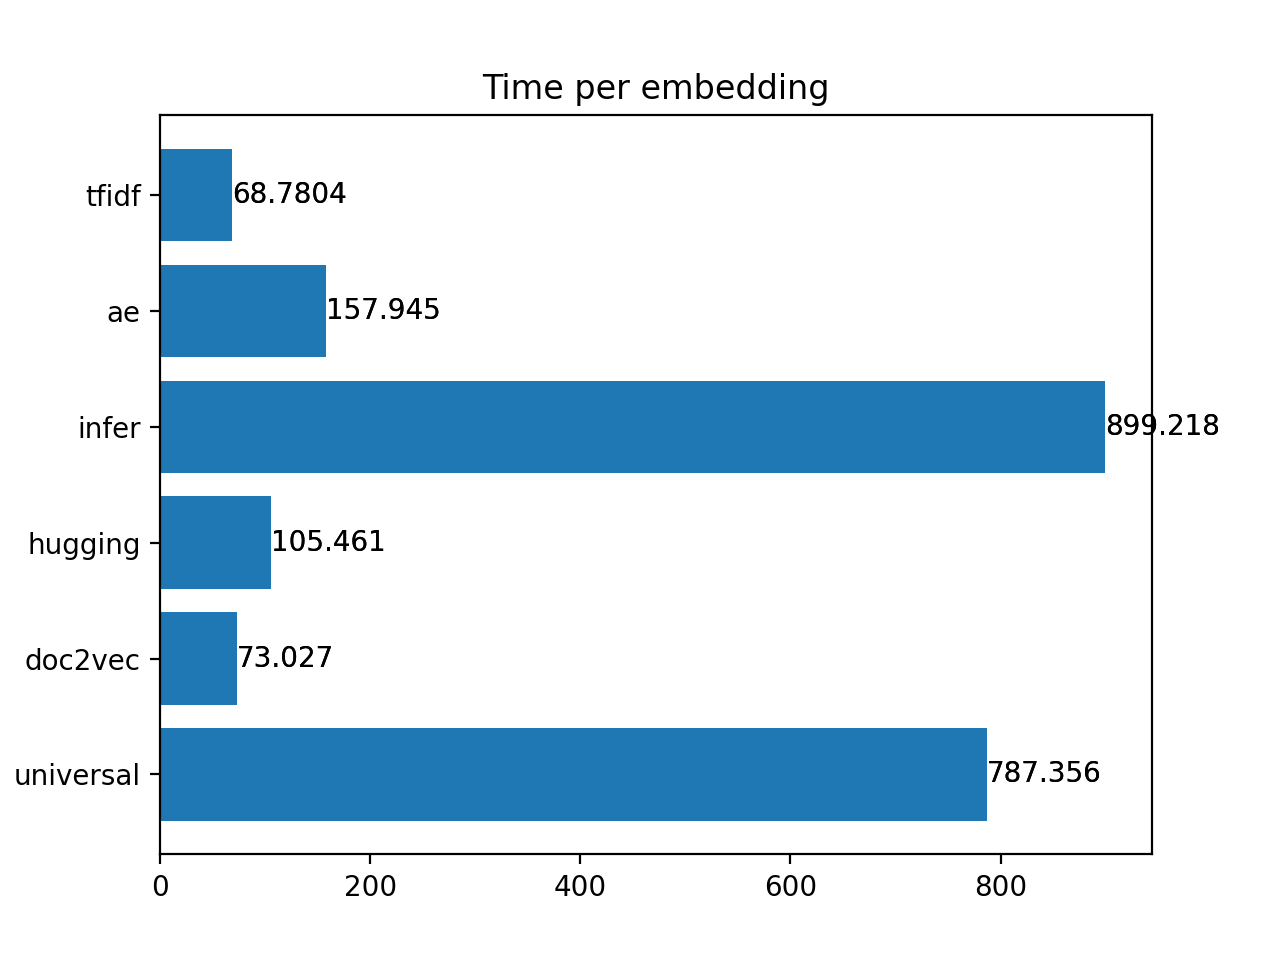
\includegraphics[width=5cm]{images/embeddings/infersent/time_per_doc_glove.png} }}%
    \qquad
    \subfloat[\centering Custom \ac{w2v} embeddings.]{{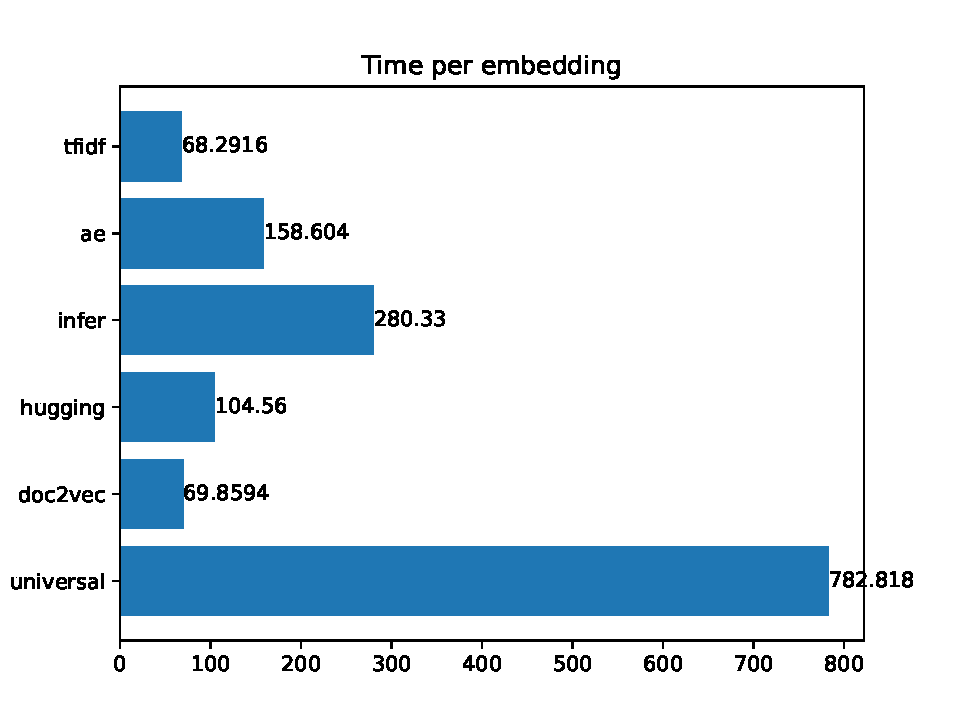
\includegraphics[width=5cm]{images/embeddings/infersent/time_per_doc_custom_emb.pdf} }}%
    \caption{Time (seconds) necessary to initialize the database, compute and insert 195 documents for specific embeddings.}%
    \label{fig:times_emb}%
\end{figure}
